$subject$=Математическая статистика
$teacher$=Лекции Блаженова А. В.
$date$=11.02.2025

\section{Лекция 1.}

Теория вероятности изучает характеристику случайных величин, тогда как математическая статистика решает обратную задачу

Допустим, что у нас есть случайная величина, по ней мы можем найти матожидание, моменты и оценить,
какое распределение имеет случайная величина. 

\subsection{Выборки}

\Def \textbf{Выборка} - набор данных, полученных в ходе экспериментов. Тогда количество экспериментов $n$ - объем Выборки

\Defs \textbf{Генеральной совокупностью} называются все результаты проведенных экспериментов

\Defs \textbf{Выборочной совокупностью} называются наблюдаемые данные экспериментов

Не все данные экспериментов мы можем наблюдать, например, выборы, тогда опросы голосовавших - выборочная совокупность, а
результаты выборов - генеральная. Очевидно, что выборочная и генеральная совокупности могут иметь различные распределения.

\Defs Выборка называется \textbf{репрезентативной}, если ее распределение близко к распределению генеральной совокупностью

Пример - \href{https://ru.wikipedia.org/wiki/%D0%A1%D0%B8%D1%81%D1%82%D0%B5%D0%BC%D0%B0%D1%82%D0%B8%D1%87%D0%B5%D1%81%D0%BA%D0%B0%D1%8F_%D0%BE%D1%88%D0%B8%D0%B1%D0%BA%D0%B0_%D0%B2%D1%8B%D0%B6%D0%B8%D0%B2%D1%88%D0%B5%D0%B3%D0%BE}{ошибка выжившего}. Во время Второй Мировой стал вопрос, в каких местах стоит бронировать корпус самолета. Самолеты 
возвращались с пулевыми отверстиям, и интуитивно казалось, что стоит бронировать те места, которые больше
всего пострадали. Однако не были учтены те самолеты, которые не вернулись, а те, которые выжили, выжили благодаря тому, что были 
прострелены в нелетальных местах, поэтому было принято решение бронировать фюзеляж в менее пострадавших местах

В дальнейшем считаем, что все выборки репрезентативны

\DefN{1} Выборкой объема $n$ называется набор из $n$ экспериментаных данных $\vec{X} = (x_1, x_2, \dots, x_n)$ (апостериорное определение)

\DefNs{2} Выборкой объема $n$ называется набор из $n$ независимых одинаково распределенных случайных
величин $\vec{X} = (X_1, X_2, \dots, X_n)$ (априорное определение)

\subsection{Выборочные характеристики}

Можно выборку рассматривать как дискретную случайную величину с одинаковыми вероятностями $p_i = \frac{1}{n}$
и вычислить для нее математическое ожидание, дисперсию и функцию распределения

\Def Выборочным средним $\overline{x}$ называется величина $\overline{x} = \frac{1}{n} \sum_{i = 1}^n X_i$

\Defs Выборочной дисперсией $D^*$ называется величина $D^* = \frac{1}{n} \sum_{i = 1}^n (X_i - \overline{x})^2$ (или $D^* = \frac{1}{n} \sum_{i = 1}^n X_i^2 - \overline{x}^2$)

По закону больших чисел выборочное среднее будет сходиться к матожиданию

\Defs Исправленной дисперсией называется величина $S^2 = \frac{n}{n - 1} D^* = \frac{1}{n - 1}\sum_{i = 1}^n (X_i - \overline{x})^2$

\hypertarget{selective_distribution_function}{}

\Def Выборочной функцией распределения $F^*(x)$ называется функция $F^*(x) = \frac{\text{число данных } x_i < x}{n}$

\begin{MyTheorem}
    \Ths Выборочная функция распределения поточечно сходится к теоретической функции распределения:

    \[\forall y \in \Real F^*(y) \overset{p}{\longrightarrow} F(y)\]
\end{MyTheorem}

\begin{MyProof}
    $F(y) = P(X < y)$

    $F^*_y = \frac{1}{n} \sum_{i = 1}^n I(X_i < y) \underset{\text{по ЗБЧ}}{\overset{p}{\longrightarrow}} EI(X_i < y) = P(X_i < y) = 
    P(X_1 < y) = F_{X_1}(y)$
\end{MyProof}

Усилим теорему

\begin{MyTheorem}
    \ThNs{Гливенко-Кантелли} $\sup_{x \in \Real} |F^*(x) - F(x)| \overset{p}{\longrightarrow} 0$
\end{MyTheorem}

\begin{MyTheorem}
    \ThNs{Колмогорова} $\sqrt{n} \sup_{x \in \Real} |F^*(x) - F(x)| \rightrightarrows K$ - распределение Колмогорова с 
    функцией распределения $F_K(x) = \sum_{j = -\infty}^{\infty} (-1)^j e^{-2 j^2 x^2}, \ x \in [0;\infty)$
\end{MyTheorem}

\hypertarget{initial_data_processing}{}

\subsection{Начальная обработка статданных}

\begin{enumerate}
    \item Ранжирование данных - упорядочиваем выборки по возрастанию. В результате получаем вариационный ряд $\vec{X} = (X_{(1)}, X_{(2)}, \dots, X_{(n)})$

    $X_{(1)} = \min X_i; \quad X_{(n)} = \max X_i$

    $X_{(i)} = i$-ая порядковая статистика

    \item Объединим повторяющиеся данные - получаем т.н. частотный вариационный ряд

    \begin{tabular}{c|c|c|c|c}
        $X_i$ & $X_{(1)}$ & \dots & $X_{(r)}$ & $\sum$ \\ 
        \hline
        $n_i$ & $n_1$ & \dots & $n_r$ & $n$ \\ 
    \end{tabular}

    Иногда часть данных отбрасывается сверху и снизу (по 5, по 10, по 5\% и так далее), чтобы сделать выборку репрезентативной

    Тогда $\overline{x} = \frac{1}{n} \sum X_i n_i$, $D^* = \frac{1}{n} \sum (X_i - \overline{x})^2 n_i$
    
    \item Чтобы уменьшить количество вычислений или сделать гистограмму, делают интервальный вариационный ряд: 
    разбиваем данные на интервалы и считаем, сколько данных $n_i$ попало в интервал. 

    Тогда $n_i$ - частота интервала $A_i$

    Есть два основные способа разбиения на интервалы: 

    \begin{enumerate}
        \item Интервалы одинаковой длины
        \item Равнонаполненные интервалы (в каждом интервале примерно одинаковое количество данных)
    \end{enumerate}

    Число интервалов $K$ такое, что $\frac{K(n)}{n} \longrightarrow 0$ и $K(n) \underset{n \to \infty}{\longrightarrow} \infty$

    Обычно применяют формулу Стерджесса $K \approx 1 + \log_2 n$ или $K \approx \sqrt[3]{n}$

    Пусть получили интервальный вариационный ряд

    \begin{tabular}{c|c|c|c|c|c}
        интервалы & $[a_0; a_1)$ & $[a_1; a_2)$ & \dots & $[a_{K - 1}; a_K]$ & $\sum$ \\ 
        \hline
        частоты & $n_1$ & $n_2$ & \dots & $n_K$ & $n$ \\ 
    \end{tabular}

\end{enumerate}

\subsection{Геометрическая интерпретация данных}

% https://www.geogebra.org/calculator/rcgr7r9f

\begin{itemize}
    \item Гистограмма

    Строится ступенчатая фигура из прямоугольников, основание $i$-ого прямоугольника - интервал, 
    высота прямоугольника - $\frac{n_i}{n l_i}$, где $l_i$ - длина интервала

    \begin{center}
        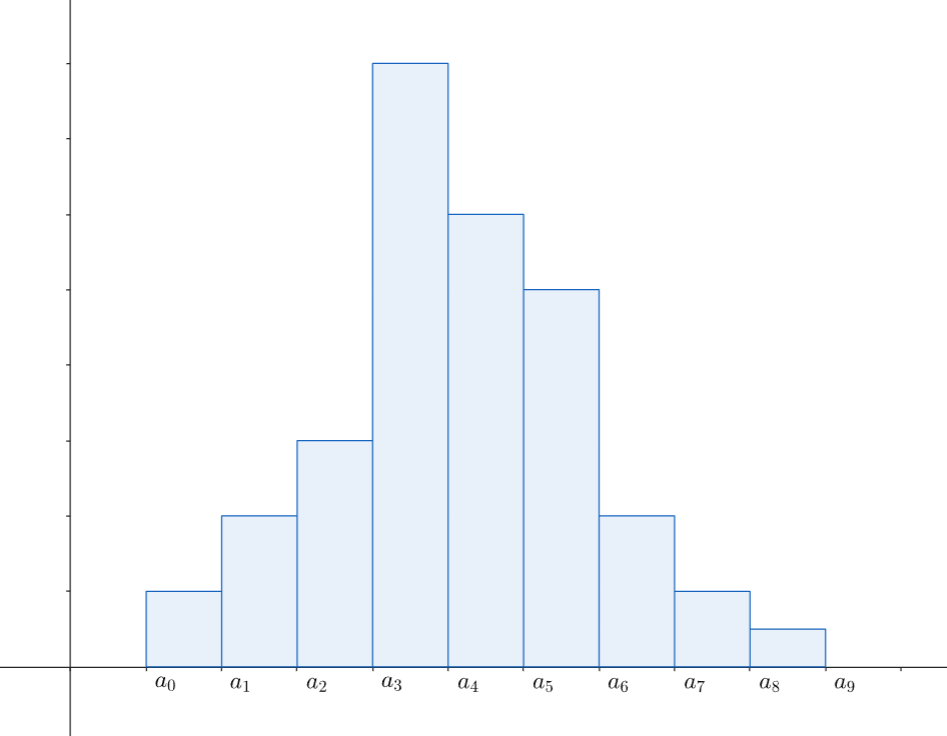
\includegraphics[width=0.7\textwidth]{mathstat/images/mathstat_2025_02_11_1}
    \end{center}

    Визуально можно сделать гипотезу, как ведет себя распределение. 

    \begin{MyTheorem}
        \Ths Гистограмма поточечно сходится к теоретической плотности
    \end{MyTheorem}

    \item Полигон

    На оси абсцисс отмечаем значения частотного вариационного ряда, по оси ординат - их частоты. 
    Получившиеся точки соединяем отрезками

    \begin{center}
        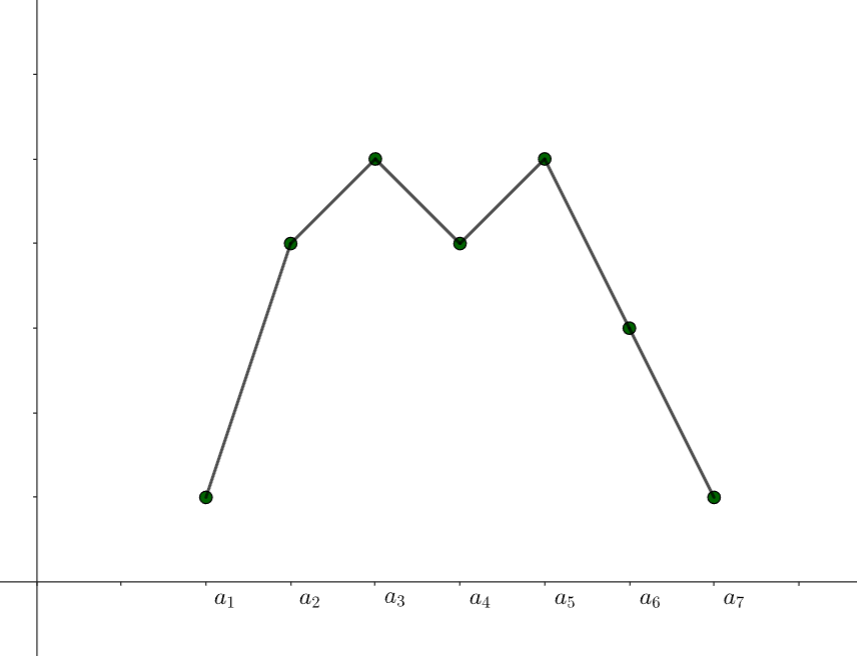
\includegraphics[width=0.7\textwidth]{mathstat/images/mathstat_2025_02_11_2}
    \end{center}

    \item Выборочная функция распределения

    На основе таблицы строится график функции распределения

    \begin{center}
        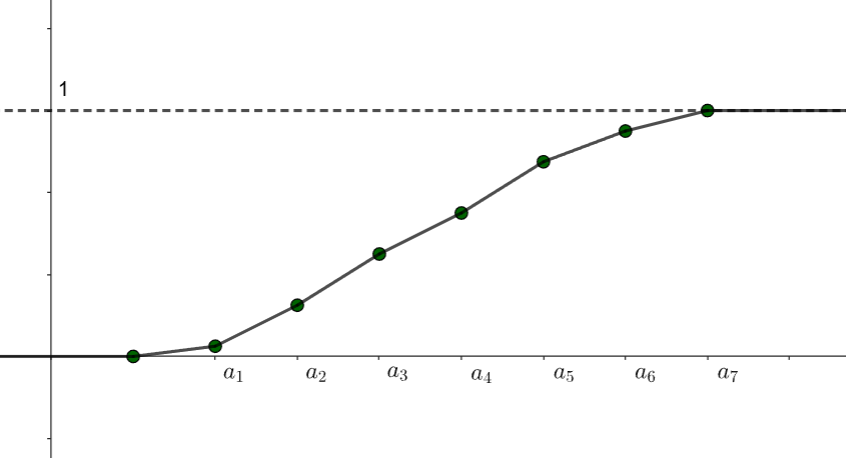
\includegraphics[width=0.7\textwidth]{mathstat/images/mathstat_2025_02_11_3}
    \end{center}

    Она может быть ступенчатой, ломаной или соединена по усмотрению

\end{itemize}




